\documentclass{article}
\raggedright
\usepackage[a4paper, hmargin=25mm, vmargin=30mm, top=20mm]{geometry}
\usepackage{color}
\usepackage{graphicx}
\usepackage{float}
\usepackage{fixltx2e}
\begin{document}
	\begin{center}
		\huge{\color{cyan}{\textbf{Archie Mittal}}
			\rule[4mm]{\textwidth}{0.5mm}}
	\end{center}
	19A/S.T.-1, Meera Vihar Apartment, \hspace{4.22cm} Contact: \mbox{+91 9453010442}\\
	A.N. Jha Marg,\hfill e-mail id: mittal.archie93@gmail.com\\
	George Town,\\
	Allahabad - 211002\\
	Uttar Pradesh\\
	\begin{figure}[h]
		\hspace{10.1cm}
		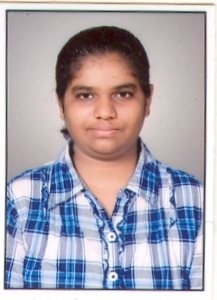
\includegraphics[scale=0.25]{Archie_Mittal.jpg}\\
	\end{figure}
	\textbf{OBJECTIVE}-To complete my project within given span of time and to succeed in an environment of growth and excellence.\\[\baselineskip]
	\textbf{EDUCATION}-
	\begin{tabular}{|c|p{5cm}|p{4cm}|p{2cm}|p{3cm}|}
		\hline
		\textbf{Degree} & \textbf{College/School} & \textbf{University} & \textbf{Passing Year} & \textbf{Pass percentage}\\
		\hline
		B.Tech. & J.K. Institute of Applied Physics \& Technology & University of Allahabad & 2017 & 81.1\% upto 1\textsuperscript{st} year\\
		\hline
		Intermediate & Girls' High School \& College & ISC & 2012 & 93.75\%\\
		\hline
		High School & Girls' High School \& College & ICSE & 2010 & 92.60\%\\
		\hline
	\end{tabular}
	\\[\baselineskip]
	\textbf{PROJECTS}-
	\begin{enumerate}
		\item
		\item
	\end{enumerate}
	\textbf{TRAINING \& INTERNSHIP}- \\
	\begin{tabular}{|p{5cm}|p{5cm}|c|p{5cm}|}
		\hline
		\textbf{Event} & \textbf{Institution} & \textbf{Year} & \textbf{Key Learning}\\
		\hline
		Core Java & Spectrum Technology & 2014 & Event Handling, GUI Applications, Multithreaded programming \\
		\hline
		Robotics Workshop & Cetpa Infotech Pvt. Ltd. & 2013 & Basics of Robotics\\
		\hline
		Science Workshop & Department of Science and Technology & 2011 & Mysteries of Space-Time, Story of Universe, Cosmology\\
		\hline
		Workshop in Aero modelling & IIIT, Allahabad & 2010 & Basic principles of aerodynamics \& history of aviation\\
		\hline
	\end{tabular}
	\\[\baselineskip]
	\textbf{RESEARCH PUBLICATIONS}-
	\begin{enumerate}
		\item
		\item 
	\end{enumerate}
	\textbf{TECHNICAL SKILLS}-
	\begin{itemize}
		\item Java Programming
		\item C Programming
		\item Basics of Robotics \\[\baselineskip]
	\end{itemize}
	\newpage
	\textbf{SOFT SKILLS}-
	\begin{enumerate}
		\item Flexible and adaptable
		\item Leadership quality 
		\item Punctual and Organised \\[\baselineskip]
	\end{enumerate}
	\textbf{EXTRA CURRICULAR ACTIVITIES}-
	\begin{itemize}
		\item 
		\item
	\end{itemize}
	\textbf{CO-CURRICULAR ACTIVITIES}-
	\\[\baselineskip]
	\begin{enumerate}
		\item 1\textsuperscript{st} prize in E-Yantra Robotics Competition 2014 conducted by IIT Bombay
		\item All India Rank-186 in Technothlon 2011 conducted by IIIT Guwahati.
		\item Bronze Medal in Individual Contest(Senior Level) in 4th International Young Mathematicians' Convention (IYMC) 2010 conducted by CMS, Lucknow.
		\item 4\textsuperscript{th} position in Commonwealth Games Quiz, 2010 conducted by History & Culture department of uniworldaim.org.
		\item 2\textsuperscript{nd} position in Java Programming Competition,2010 organised by Girls' High School \& College.
		\item 49\textsuperscript{th} position in TSI Maths Olympiad,2008.
		\item Percentile score 74.07\% in Global Mathematical Talent Probe,2008 conducted by Institute for Scholastic Evaluation.\\[\baselineskip]
	\end{enumerate}
	\textbf{PERSONAL DETAILS}- \\
	\textbf{Father's Name:} Mr. Alok Mittal\\
	\textbf{Mother's Name:} Mrs. Preeti Mittal\\
	\textbf{Sex:} Female\\
	\textbf{Date Of Birth:} 10 December, 1993\\
	\textbf{Nationality:} Indian\\
	\textbf{Marital Status:} Single\\[\baselineskip]
\end{document}